\documentclass[a4paper,10pt]{article}

\usepackage[utf8]{inputenc}
\usepackage{subfig}
\usepackage{graphicx}

\def\sun{\hbox{$\odot$}}
\def\farcs{\hbox{$.\!\!^{\prime\prime}$}}
\newcommand{\hvol}{h^{3}{\mathrm{Mpc}}^{-3}}
\newcommand{\hmpc}{\ensuremath{h^{-1}\mathrm{Mpc}}}
\newcommand{\hkpc}{\ensuremath{h^{-1}\mathrm{kpc}}}
\newcommand{\hMsun}{h^{-1}M_{\odot}}
\newcommand{\Msun}{M_{\odot}}
\newcommand{\kms}{{\,{\rm km}\,{\rm s}^{-1}}}
\newcommand{\Omegam}{\Omega_{m}}
\newcommand{\Omegab}{\Omega_{b}}
\newcommand{\Omegal}{\Omega_{\Lambda}}
\newcommand{\xig}{\xi_{\rm gg}(r)}
\newcommand{\xih}{\xi_{\rm hh}(r)}
\newcommand{\xim}{\xi_{\rm mm}(r)}
\newcommand{\ds}{\ensuremath{\Delta\Sigma}}
\newcommand{\scinv}{\ensuremath{\Sigma_c^{-1}}}
\newcommand{\avgscinv}{\ensuremath{\langle\Sigma_c^{-1}\rangle}}
\newcommand{\hinvk}{$h^{-1}$kpc}
\newcommand{\avgnm}{\ensuremath{\langle N(M)\rangle}}
\newcommand{\fclust}{\ensuremath{f_\mathrm{clust}}}
\newcommand{\fbcg}{\ensuremath{f_\mathrm{BCG}}}

% upright d in integrals
\newcommand{\rmd}{\mathrm{d}}
\newcommand{\putcite}{\textbf{(CITE)}}
\newcommand{\ic}{\ensuremath{I_\mathrm{C}}}
\newcommand{\pc}{\ensuremath{G_\mathrm{C}}}
\newcommand{\ps}{\ensuremath{G_\mathrm{T}}}
\newcommand{\tic}{\ensuremath{\tilde{I}_\mathrm{C}}}
\newcommand{\tpc}{\ensuremath{\tilde{G}_\mathrm{C}}}
\newcommand{\tps}{\ensuremath{\tilde{G}_\mathrm{T}}}
\newcommand{\tkpd}{\ensuremath{\tilde{T}}}
\newcommand{\ticpd}{\ensuremath{\tilde{P}}}
\newcommand{\ticpdr}{\ensuremath{\tilde{P}^\mathrm{(rot)}}}
\newcommand{\ticpds}{\ensuremath{\tilde{P}^{(\gamma)}}}
\newcommand{\ticpdrs}{\ensuremath{\tilde{P}^{(\mathrm{rot},\gamma)}}}
\newcommand{\tks}{\ensuremath{\tilde{K}_\mathrm{T}}}
\newcommand{\tksr}{\ensuremath{\tilde{K}_\mathrm{T}^\mathrm{(rot)}}}
\newcommand{\tis}{\ensuremath{\tilde{I}^{(\gamma)}_\mathrm{T}}}
\newcommand{\tisr}{\ensuremath{\tilde{I}^{(\mathrm{rot},\gamma)}_\mathrm{T}}}
\newcommand{\is}{\ensuremath{I_\mathrm{T}}}
\newcommand{\isr}{\ensuremath{I_\mathrm{T}^\mathrm{(rot)}}}
\newcommand{\rpix}{\ensuremath{R_\mathrm{pix}}}
\newcommand{\nimg}{\ensuremath{N_\mathrm{img}}}
\newcommand{\nrand}{\ensuremath{N_\mathrm{rand}}}
\newcommand{\nset}{\ensuremath{N_\mathrm{set}}}
\newcommand{\nc}{\ensuremath{N_\mathrm{C}}}
\newcommand{\ns}{\ensuremath{N_\mathrm{S}}}
\newcommand{\nt}{\ensuremath{N_\mathrm{T}}}
\newcommand{\erms}{\ensuremath{e_\mathrm{rms}}}
\newcommand{\etot}{\ensuremath{e_\mathrm{tot}}}
%\newcommand{\newtext}{\emph}
\newcommand{\newtext}{}
\newcommand{\reftext}[1]{\textbf{#1}}

%More new commands by Arun Kannawadi
\newcommand{\mg}{\ensuremath{M_G} }
\newcommand{\mi}{\ensuremath{M_I} }

%opening
\title{Redshift analysis of Sersic $n$}
\author{Arun Kannawadi Jayaraman}

\textwidth=6.4in
\textheight=8.7in
\oddsidemargin=0.0in
\evensidemargin=0.0in
\topmargin=-0.8in
\addtolength\topmargin{0.6in}
\marginparwidth 0.75in
\marginparsep 7pt

\begin{document}

\maketitle

It is good to have this overdensity vs redshift plot handy and hence I attach it here. \\

\begin{figure}
 \centering
  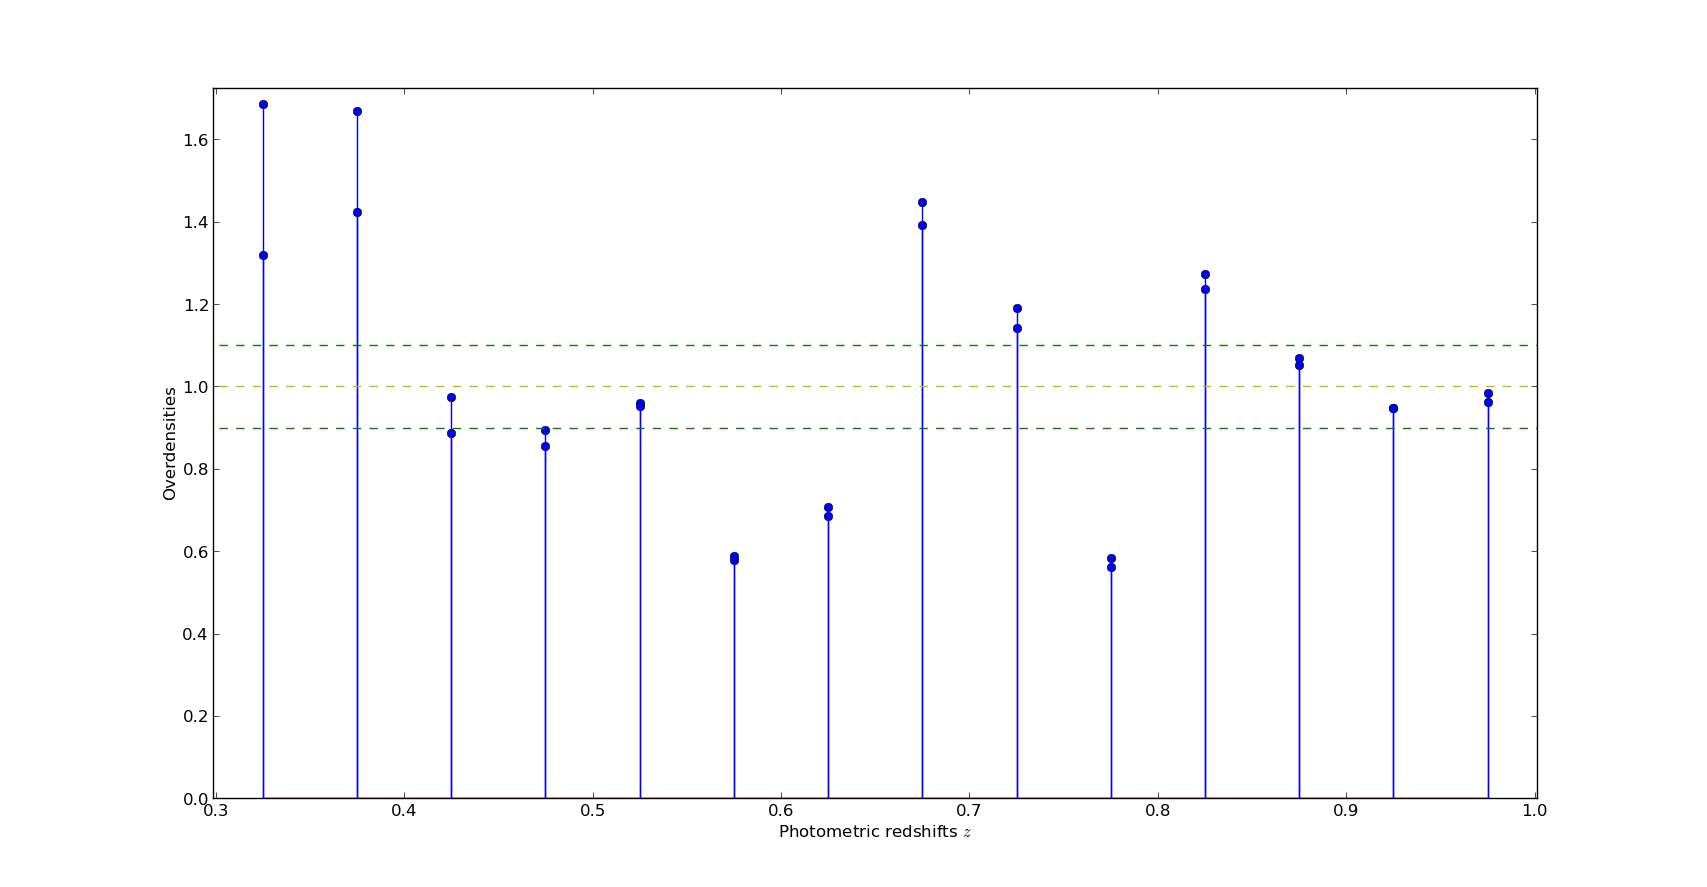
\includegraphics[scale=0.25]{overdensities.png}
\end{figure}

In all the plots that follow, I have both the histogram and the CDF obtained from the histogram plotted so that we can easily see where the difference comes from.
It also explains why truncation of Sersic $n$ values at 6 doesn't affect our analysis much.

\pagebreak
\section{All overdense and underdense regions}
Here is a comparison of Sersic $n$ of all overdense regions i.e. $z=[0.3-0.4] \cup [0.65-0.75] \cup [0.80-0.85]$ and all underdense regions
i.e. $z=[0.55-0.65]\cup[0.75-0.80]$.
\begin{figure}[ht]
 \centering
  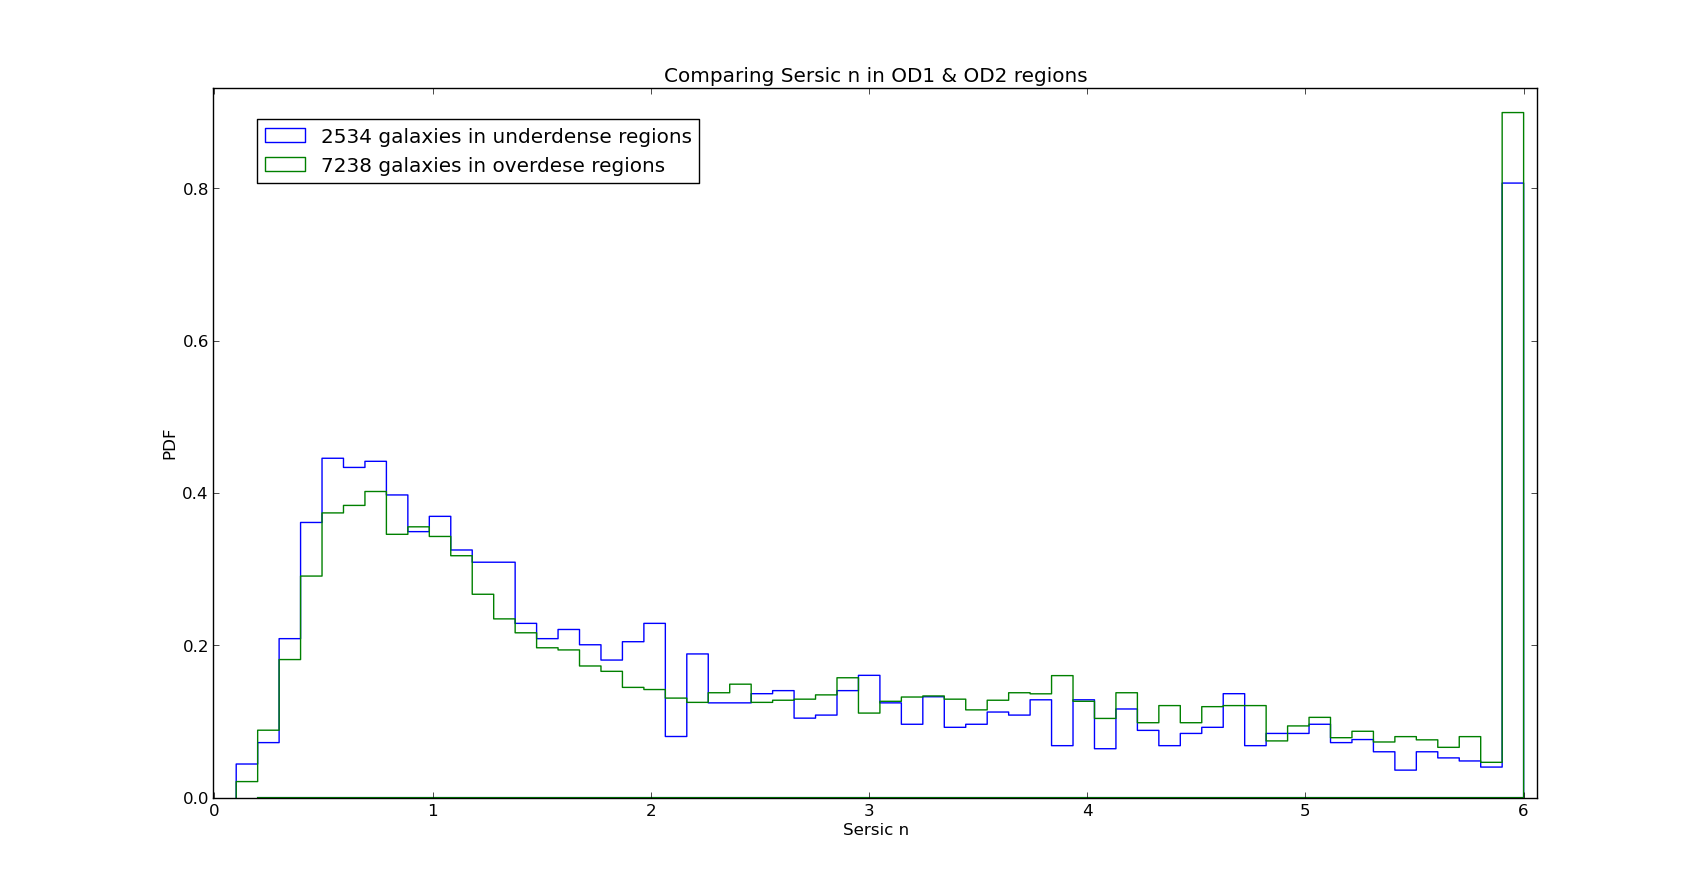
\includegraphics[scale=0.3]{hist_sersicn_ODUD.png}
  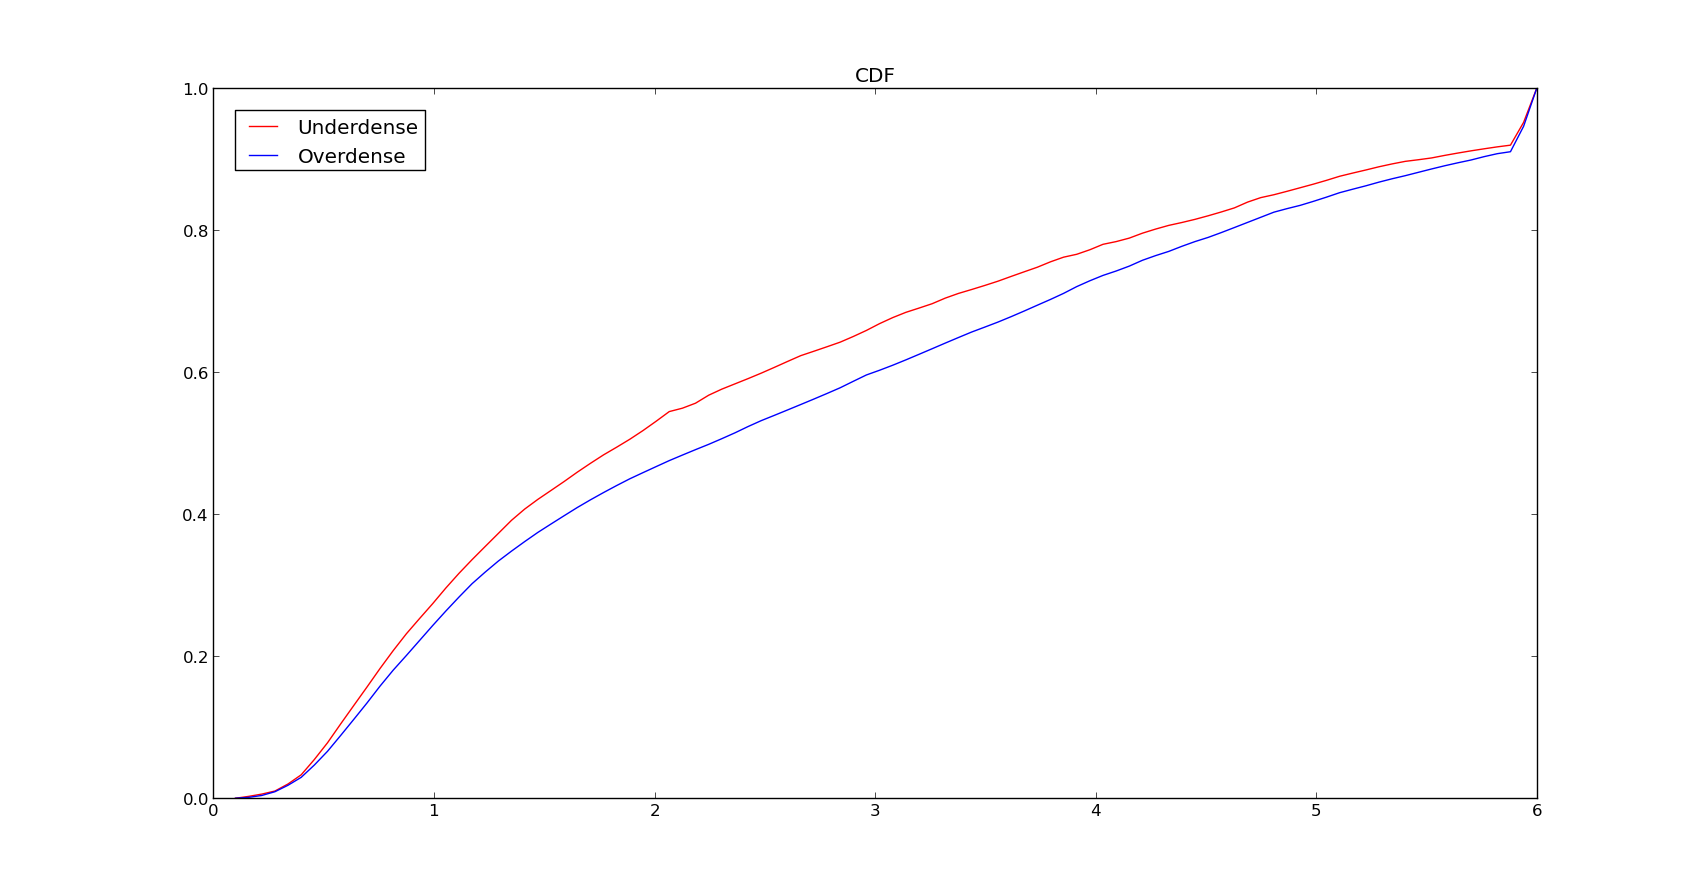
\includegraphics[scale=0.3]{cdf_sersicn_ODUD.png}
\end{figure}

\pagebreak 
\section{Nearby overdense regions}
Here we compare the two nearby overdense regions $z=0.65-0.70$ and $0.70-0.75$.

\begin{figure}[ht]
 \centering
 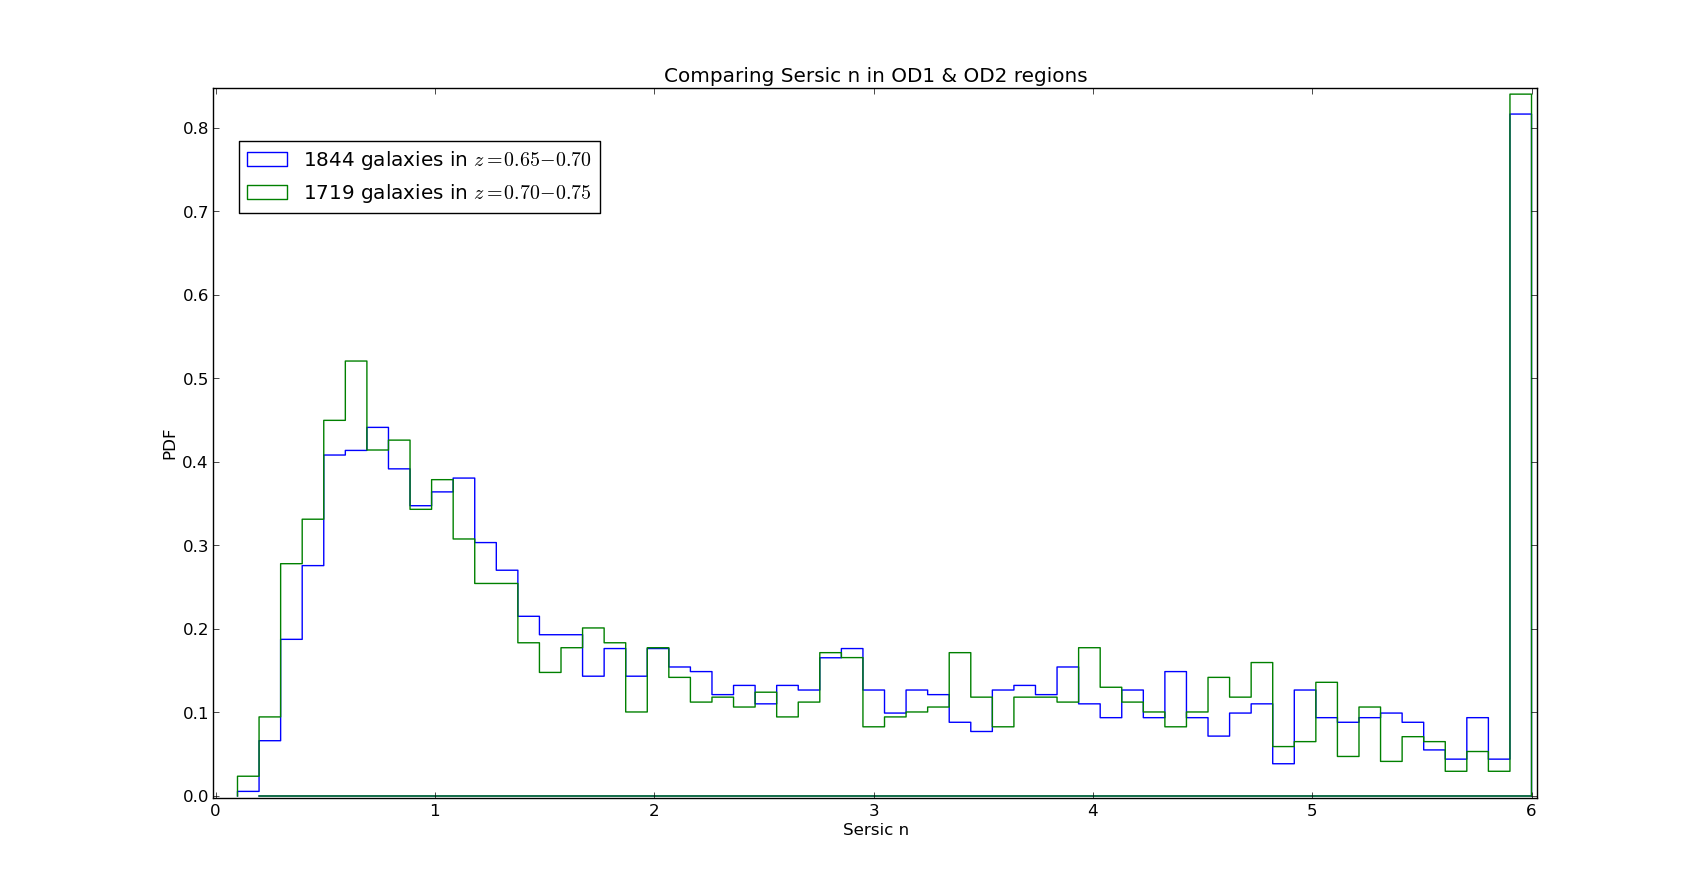
\includegraphics[scale=0.3]{hist_sersicn_ODOD.png}
 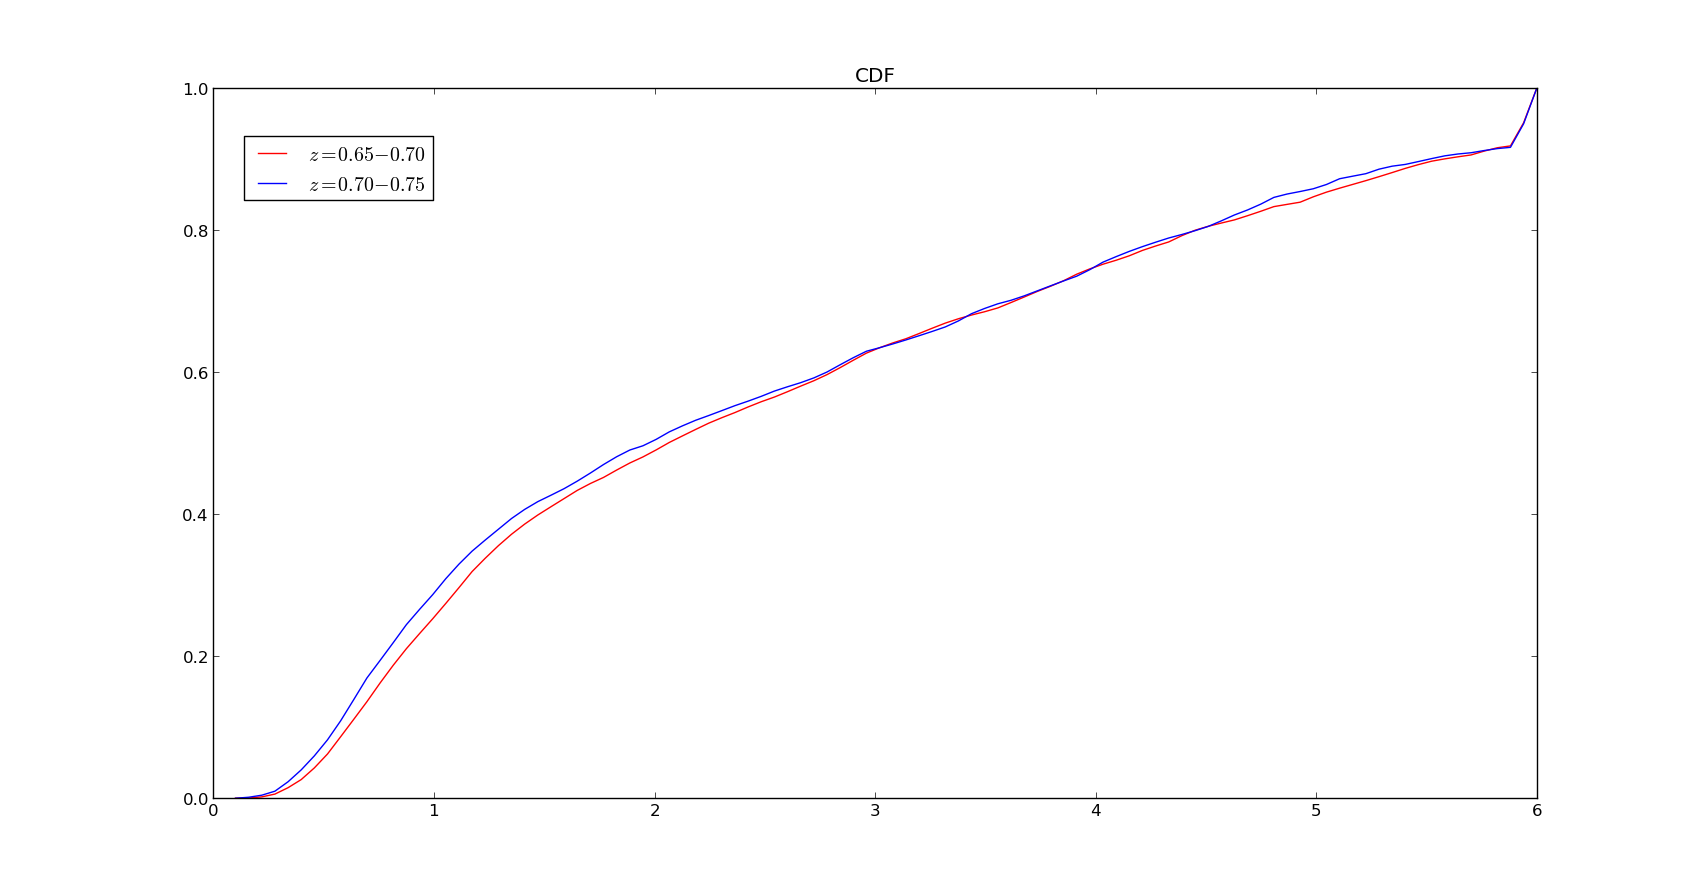
\includegraphics[scale=0.3]{cdf_sersicn_ODOD.png}
 \caption{KS p-value = 0.1397 \& AD p-value = 0.07405}
 
\end{figure}

\pagebreak 
\section{Nearby overdense and underdense regions}
Here we compare the overdense region $z=0.65-0.75$ and its neighbouring underdense region $z=0.55-0.65$. Note that the overdensity values
of these regions significantly differ.

\begin{figure}[ht]
 \centering
 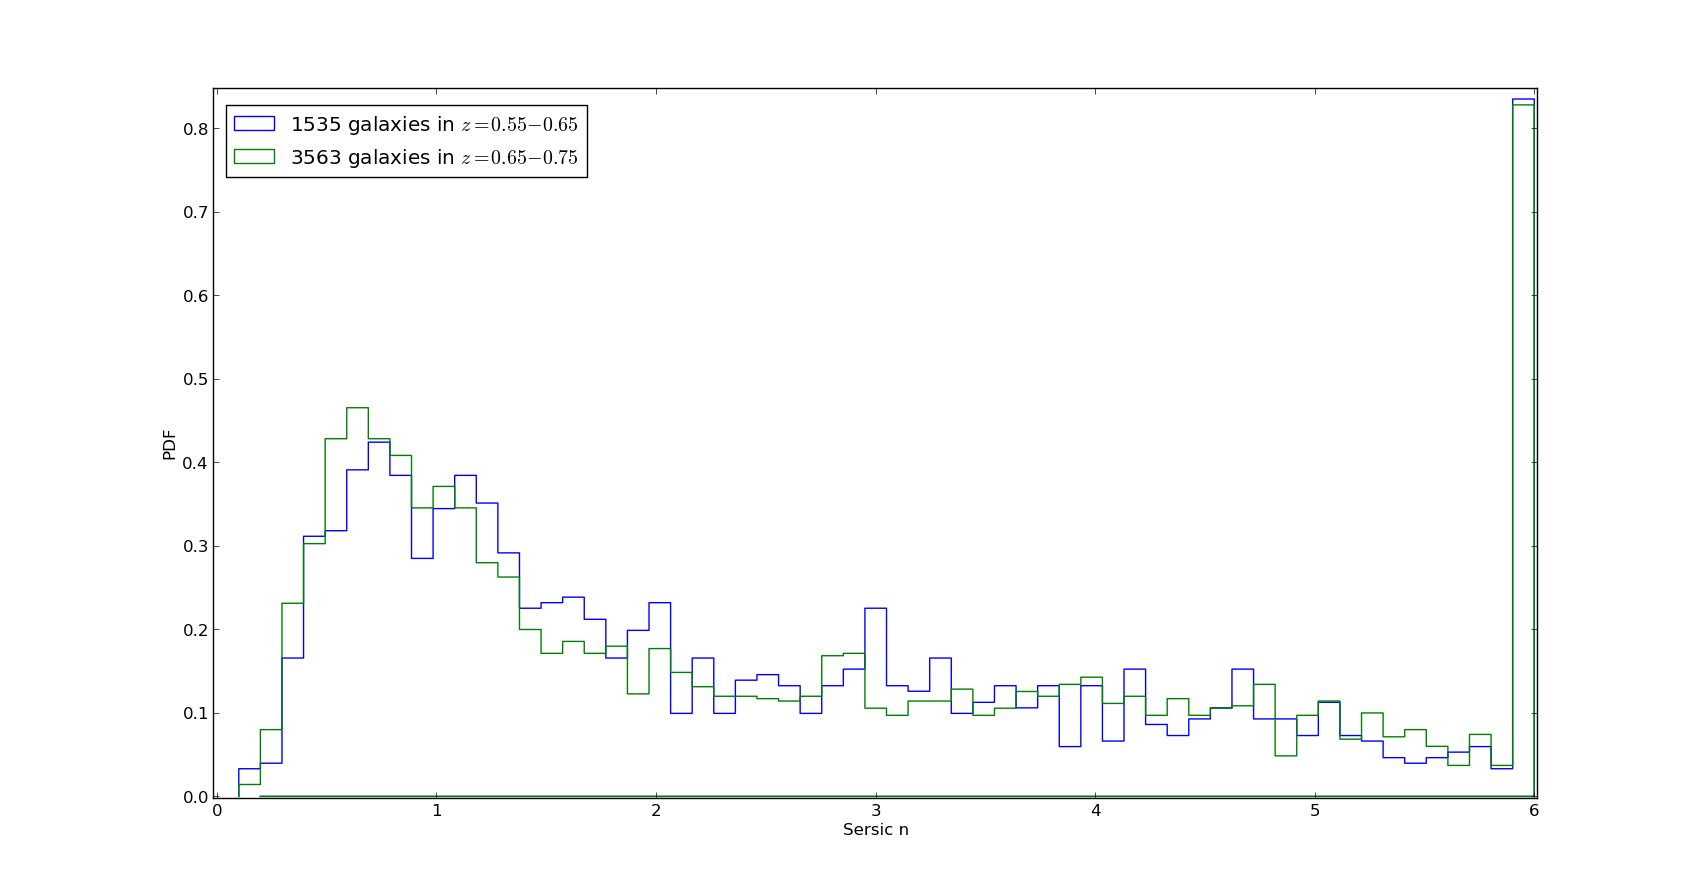
\includegraphics[scale=0.35]{hist_sersicn_ODUD(2).png}
 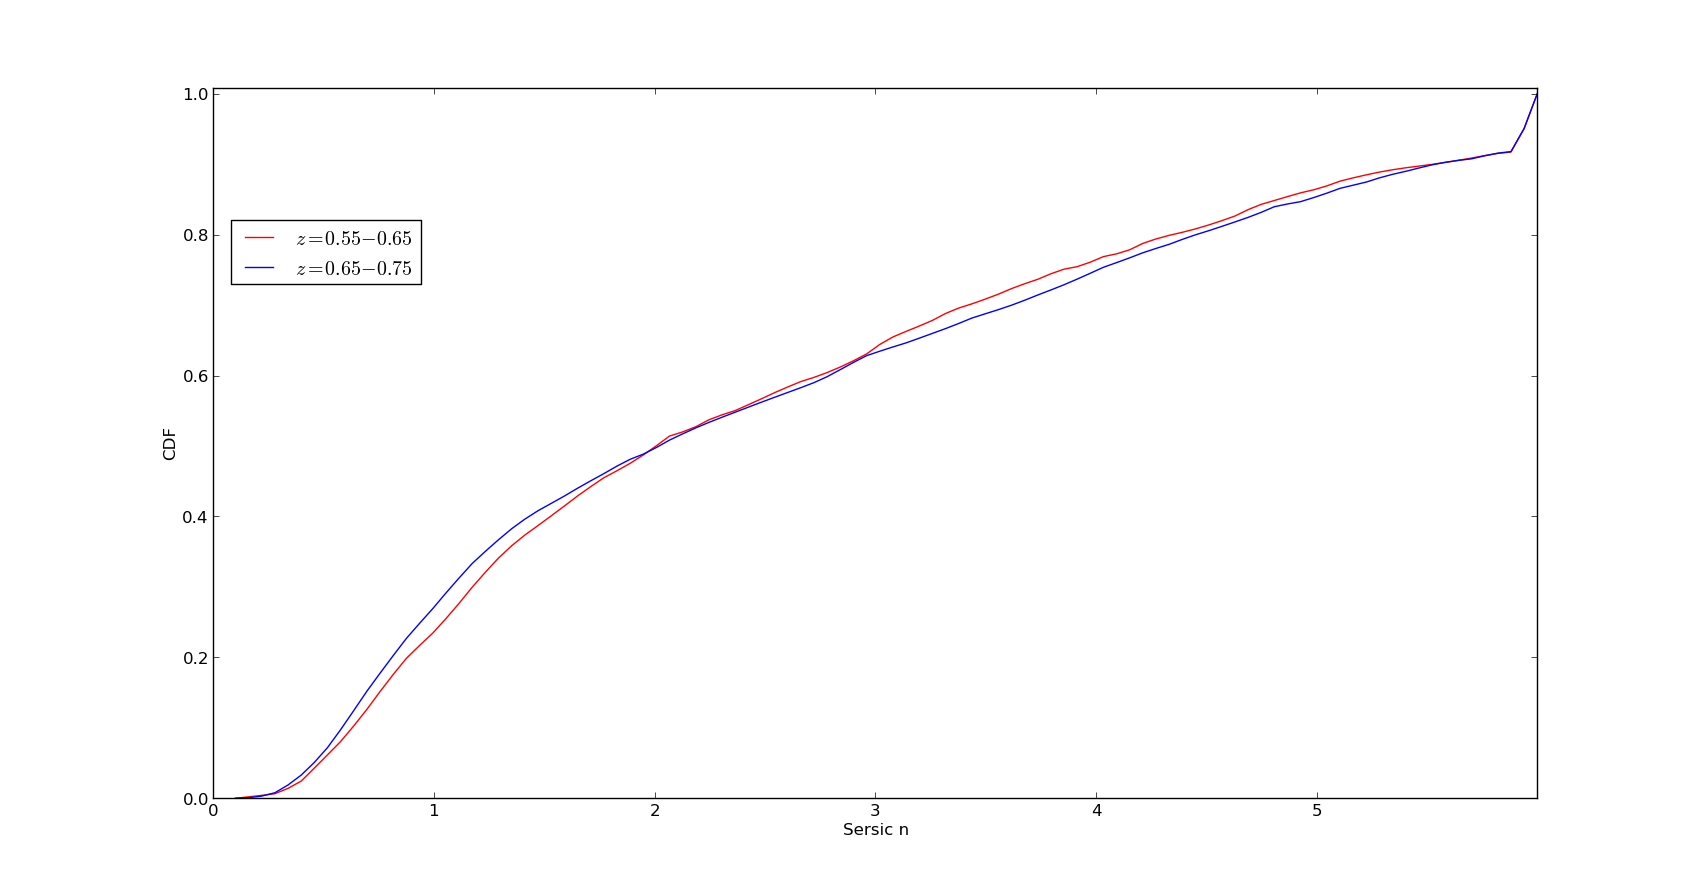
\includegraphics[scale=0.35]{cdf_sersicn_ODUD(2).png}
 \caption{KS p-value = 0.0606 \& AD p-value = 0.0402}
\end{figure} 

If we narrow our redshift ranges and look at the underdense $z=0.60-0.65$ and the overdense $z=0.65-0.70$ bins \pagebreak

\begin{figure}[ht]
 \centering
 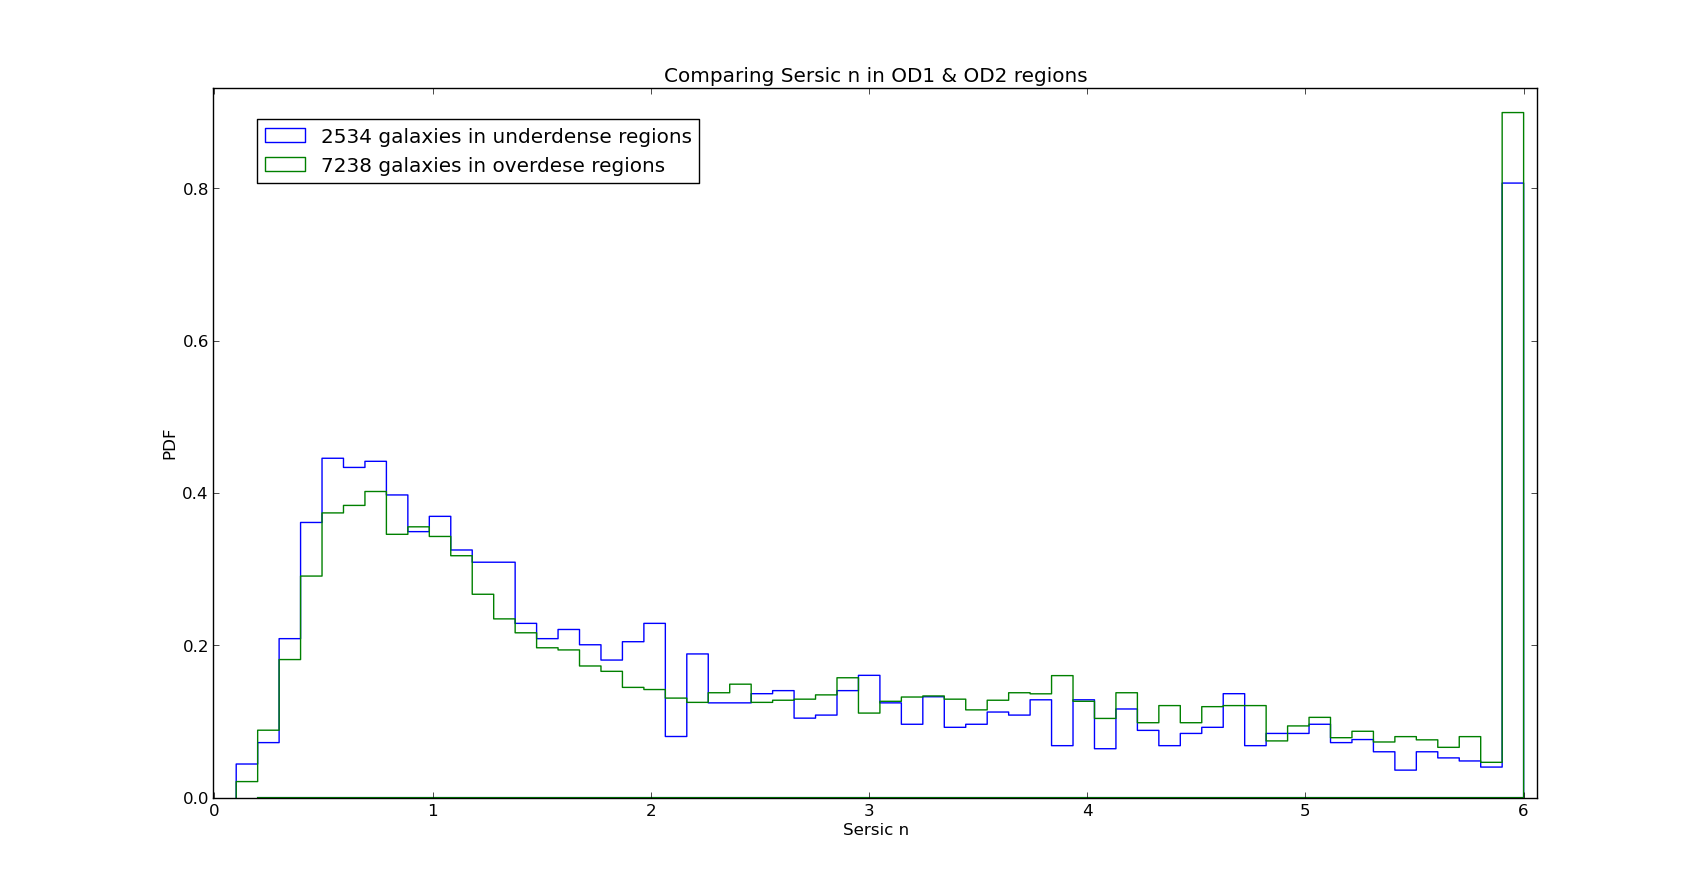
\includegraphics[scale=0.3]{hist_sersicn_ODUD.png}
 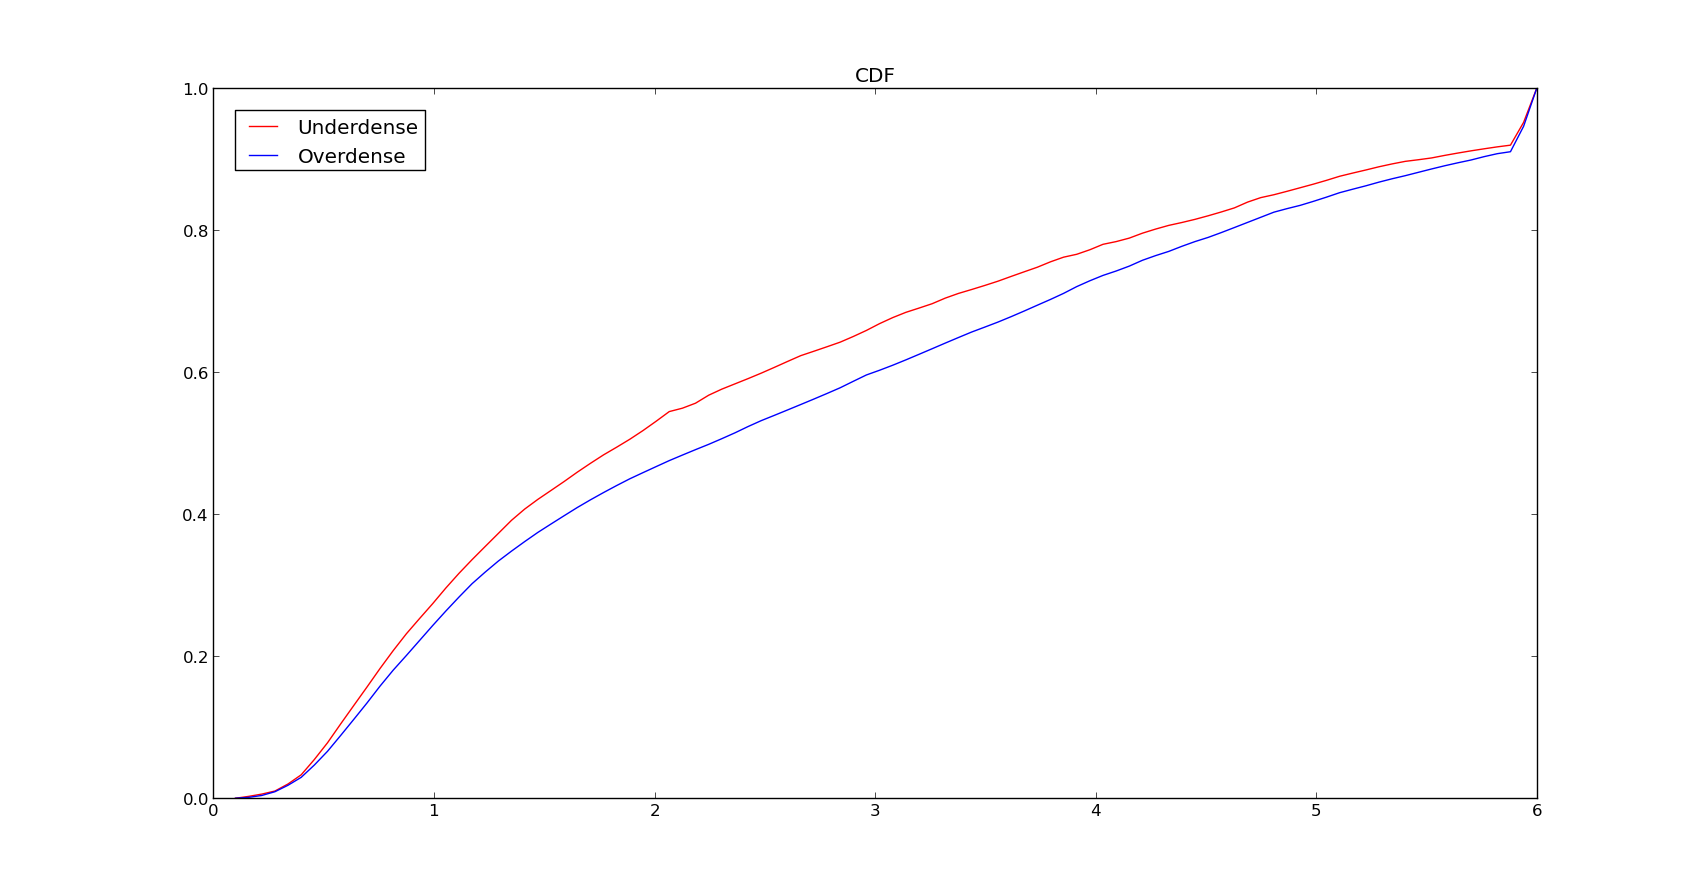
\includegraphics[scale=0.3]{cdf_sersicn_ODUD.png}
 \caption{KS p-value = 0.3895 \& AD p-value = 0.4831}
\end{figure}

The high p-values maybe are reflecting the mixing of galaxies in overdense and underdense regions due to errors in redshifts.

\pagebreak
\section{Low $z$ and High $z$ comparison}
\begin{figure}[ht]
 \centering
  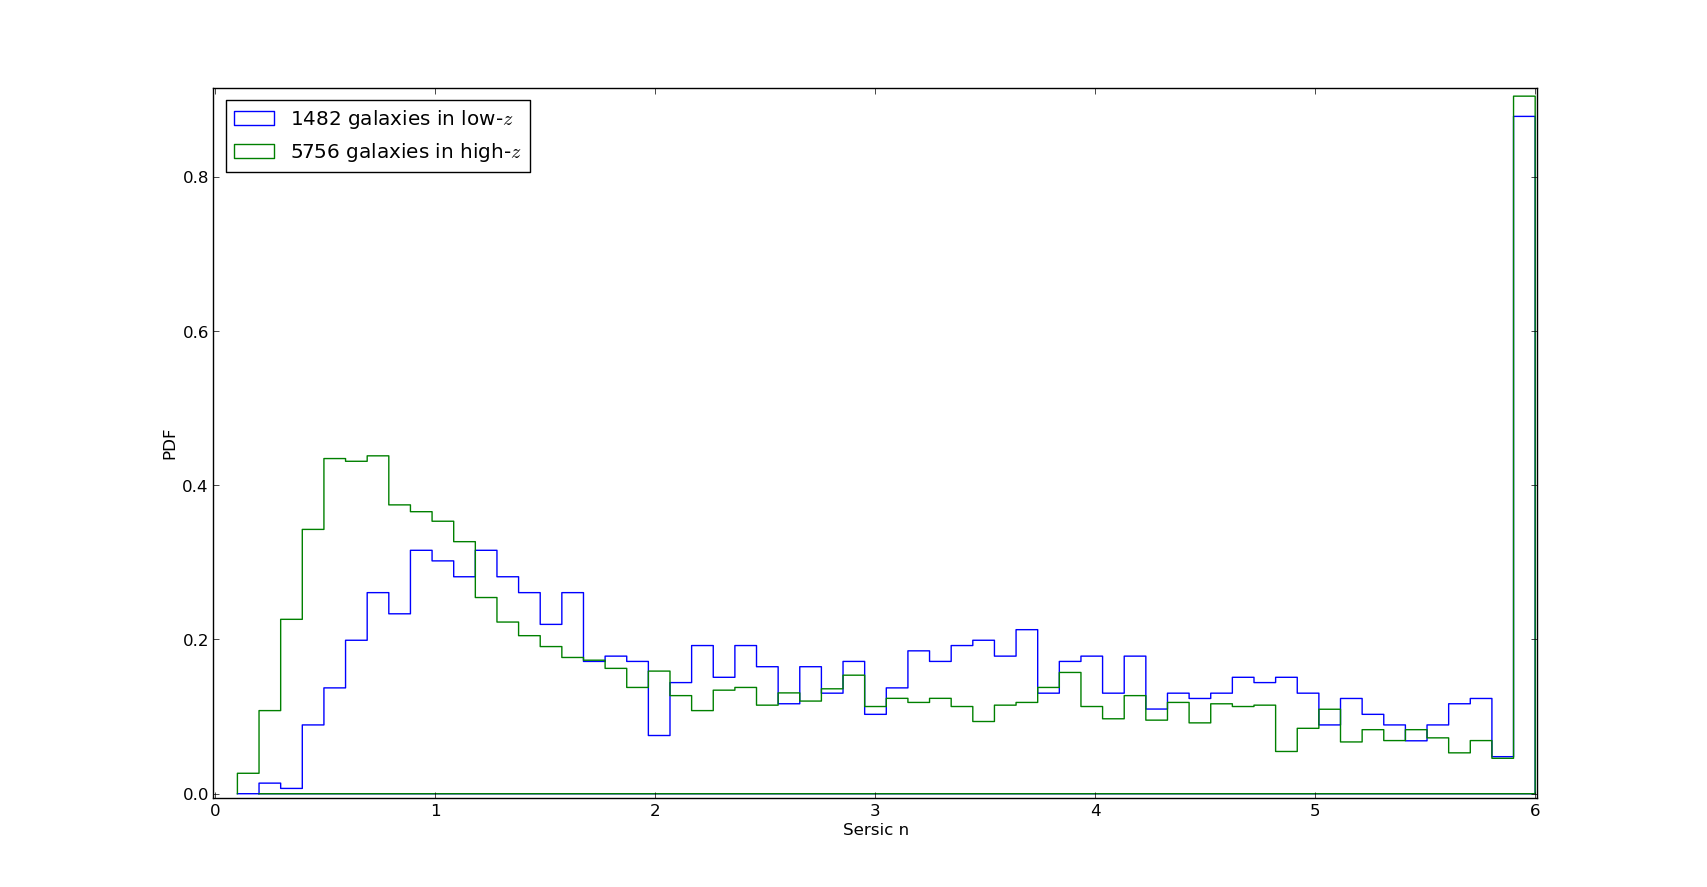
\includegraphics[scale=0.3]{hist_sersicn_LowHighZ.png}
  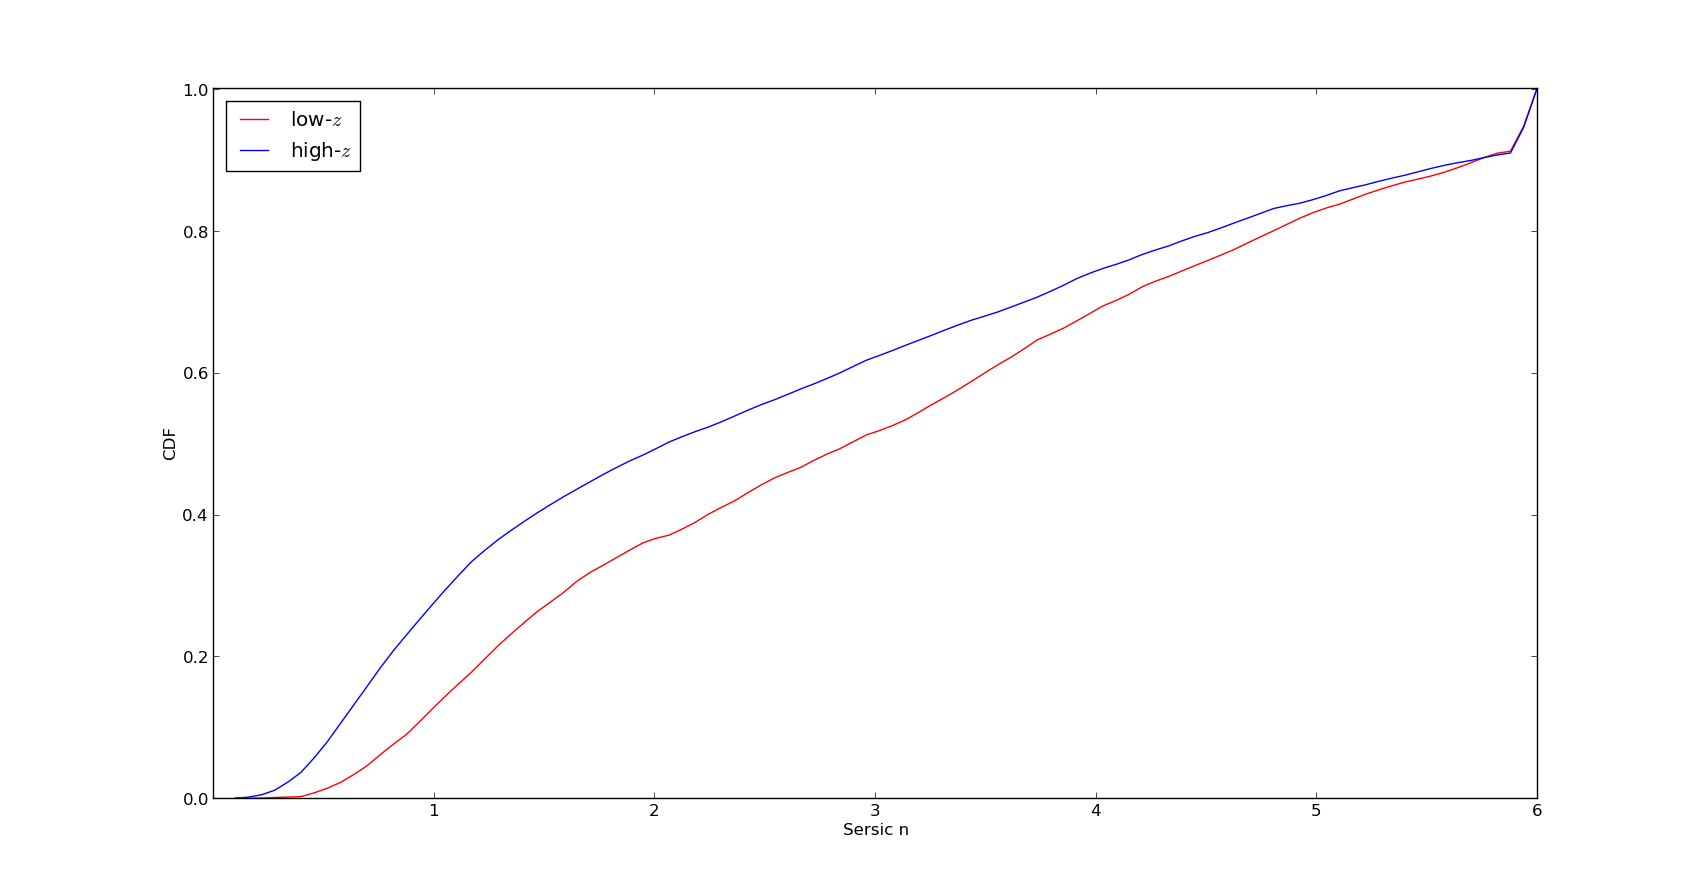
\includegraphics[scale=0.3]{cdf_sersicn_LowHighZ.png}
  \caption{KS p-value = 2.6e-26 \& AD p-value = 0.0 \\ KS statistic = 0.1584 \& AD statistic = 83.059}
\end{figure}

\section{Comments}
So we've seen earlier that the Sersic $n$ distributions of all overdense and underdense regions put together are inconsistent and that
randomly partitioning galaxies in overdense regions fairly agree with each other. From the section above, we see a clear disagreement when 
we consider the overdense regions in low-$z$ region when compared to a high-$z$ overdense region, which suggests there may be some
evolution with redshift. Galaxies at larger redshifts tend to have lower Sersic $n$ values. 

The random partitioning of galaxies in overdense regions wash away any redshift dependence. But the incosistency in comparing
all overdense and underdense regions might be partially due to inherent differences and partly due to redshift dependence.
\end{document}
